\documentclass{article}

\usepackage[dvipsnames]{xcolor}
\usepackage{hyperref}
\definecolor{COLOR_MEAN}{HTML}{f0f0f0}
\definecolor{LINK_COLOR}{HTML}{636EFA}
\hypersetup{
	colorlinks=true,
	linkcolor=LINK_COLOR,
	urlcolor=LINK_COLOR,
	citecolor=LINK_COLOR,
}

% if you need to pass options to natbib, use, e.g.:
%     \PassOptionsToPackage{numbers, compress}{natbib}
% before loading neurips_2024


% ready for submission
%\usepackage{neurips_2024}


% to compile a preprint version, e.g., for submission to arXiv, add add the
% [preprint] option:
% \usepackage[preprint]{neurips_2024}


% to compile a camera-ready version, add the [final] option, e.g.:
\usepackage[final]{neurips_2024}


% to avoid loading the natbib package, add option nonatbib:
%    \usepackage[nonatbib]{neurips_2024}


\usepackage[utf8]{inputenc} % allow utf-8 input
\usepackage[T1]{fontenc}    % use 8-bit T1 fonts
\usepackage{hyperref}       % hyperlinks
% \usepackage{url}            % simple URL typesetting
\usepackage{xurl}
\usepackage{booktabs}       % professional-quality tables
\usepackage{amsfonts}       % blackboard math symbols
\usepackage{nicefrac}       % compact symbols for 1/2, etc.
\usepackage{microtype}      % microtypography
\usepackage{xcolor}         % colors
\usepackage{tabularx}
\usepackage{booktabs}
\usepackage{amsmath}
\usepackage{listings}
\usepackage{xspace}
\usepackage{cleveref}
\usepackage{multirow}
\usepackage{multicol}
\usepackage{subcaption}
\usepackage{placeins}

\usepackage{algorithm} 
\usepackage{algpseudocode}
\usepackage{mathrsfs}
\usepackage{tikz}
\usepackage{listings}

\usepackage[symbol]{footmisc}
\definecolor{ntured}{HTML}{D71440}
\hypersetup{
    colorlinks=true,     
    urlcolor=ntured,
}

\lstset{ 
  language=R,                     % the language of the code
  basicstyle=\ttfamily, % the size of the fonts that are used for the code
  numbers=left,                   % where to put the line-numbers
  numberstyle=\color{Blue},  % the style that is used for the line-numbers
  stepnumber=1,                   % the step between two line-numbers. If it is 1, each line
                                  % will be numbered
  numbersep=5pt,                  % how far the line-numbers are from the code
  backgroundcolor=\color{white},  % choose the background color. You must add \usepackage{color}
  showspaces=false,               % show spaces adding particular underscores
  showstringspaces=false,         % underline spaces within strings
  showtabs=false,                 % show tabs within strings adding particular underscores
  frame=single,                   % adds a frame around the code
  rulecolor=\color{black},        % if not set, the frame-color may be changed on line-breaks within not-black text (e.g. commens (green here))
  tabsize=2,                      % sets default tabsize to 2 spaces
  captionpos=b,                   % sets the caption-position to bottom
  breaklines=true,                % sets automatic line breaking
  breakatwhitespace=false,        % sets if automatic breaks should only happen at whitespace
  keywordstyle=\color{RoyalBlue},      % keyword style
  commentstyle=\color{YellowGreen},   % comment style
  stringstyle=\color{ForestGreen}      % string literal style
} 




\title{MH3511 Regression Analysis}


% The \author macro works with any number of authors. There are two commands
% used to separate the names and addresses of multiple authors: \And and \AND.
%
% Using \And between authors leaves it to LaTeX to determine where to break the
% lines. Using \AND forces a line break at that point. So, if LaTeX puts 3 of 4
% authors names on the first line, and the last on the second line, try using
% \AND instead of \And before the third author name.


% \author{
% }

\usepackage{graphicx}
\usepackage{tablefootnote}

\begin{document}
	
\begin{titlepage}
	\begin{figure}[!t]
		\centering
		
\includegraphics[width = 4.3in]{title/logo.pdf}
	\end{figure}
	
	\centering
	\huge{\textbf{MH3510 Regression Analysis}}\\[0.2in]
	\huge{\textbf{Group Project}}\\[2in]
	
	%	\LARGE{\textbf{YOUR NAME}}\\
	%	\normalsize{Matriculation number}\\[0.2in]
	
	\begin{table}[h]
		\centering
		\resizebox{\textwidth}{!}{%
			\begin{tabular}{|l|l|l|} \hline 
				
				\textbf{Name} & \textbf{Email} & \textbf{Matric Number} \\ \hline 
				
				Pu Fanyi & \texttt{FPU001@e.ntu.edu.sg} & \texttt{U2220175K} \\ \hline 
				Shan Yi & \texttt{SH0005YI@e.ntu.edu.sg} & \texttt{U2222846C}\\ \hline 
                    Zhang Kaichen & \texttt{ZHAN0564@e.ntu.edu.sg} & \texttt{U2123722J} \\ \hline 
                    Mu Yichen & \texttt{M220100@e.ntu.edu.sg} & \texttt{U2240144L} \\ \hline 
				
 Fu Yilin& \texttt{FUYI0005@e.ntu.edu.sg}&\texttt{U2240718G}\\ \hline
			\end{tabular}%
		}
	\end{table}

	
	
    
	
	%	\large{A Final Year Report submitted to Asian School of the Environment, Nanyang Technological University in partial fulfilment of the requirements for the Degree of }\\[0.1in]
	
	\vspace{0.5in}
	\LARGE{Nanyang Technological University, Singapore}\\[0.3in]	
	
	\LARGE{2024/2025 Semester 1}
	\newpage
\end{titlepage}

\suppressfloats[t]

\section{Introduction}

In this study, we investigate factors affecting Annual Average Daily Traffic (AADT) on road section, using a dataset comprising five variables shown in Table \ref{tab:variable_overview}. We demonstrate our overall pipeline in Figure \ref{fig:intro}. After inputting our data, we first observe its distribution. To address the skewness in some of the data, we applied transformations to the data. 

After that, we conduct Single Linear Regression (SLR) analysis for $x_1$ to $x_4$. We analyze and explain the influence of each variable on the response variable in detail through this approach. In parallel, we also perform Multiple Linear Regression (MLR) analysis to get the more precise model. For variables found to be significant, we proceed to use them for prediction.

The full code can be reached in \url{https://pufanyi.github.io/MH3510-Project/}, we also listed some key code snips in Appendix \ref{appendix:key_code}.

\begin{figure}[t]
    \centering
    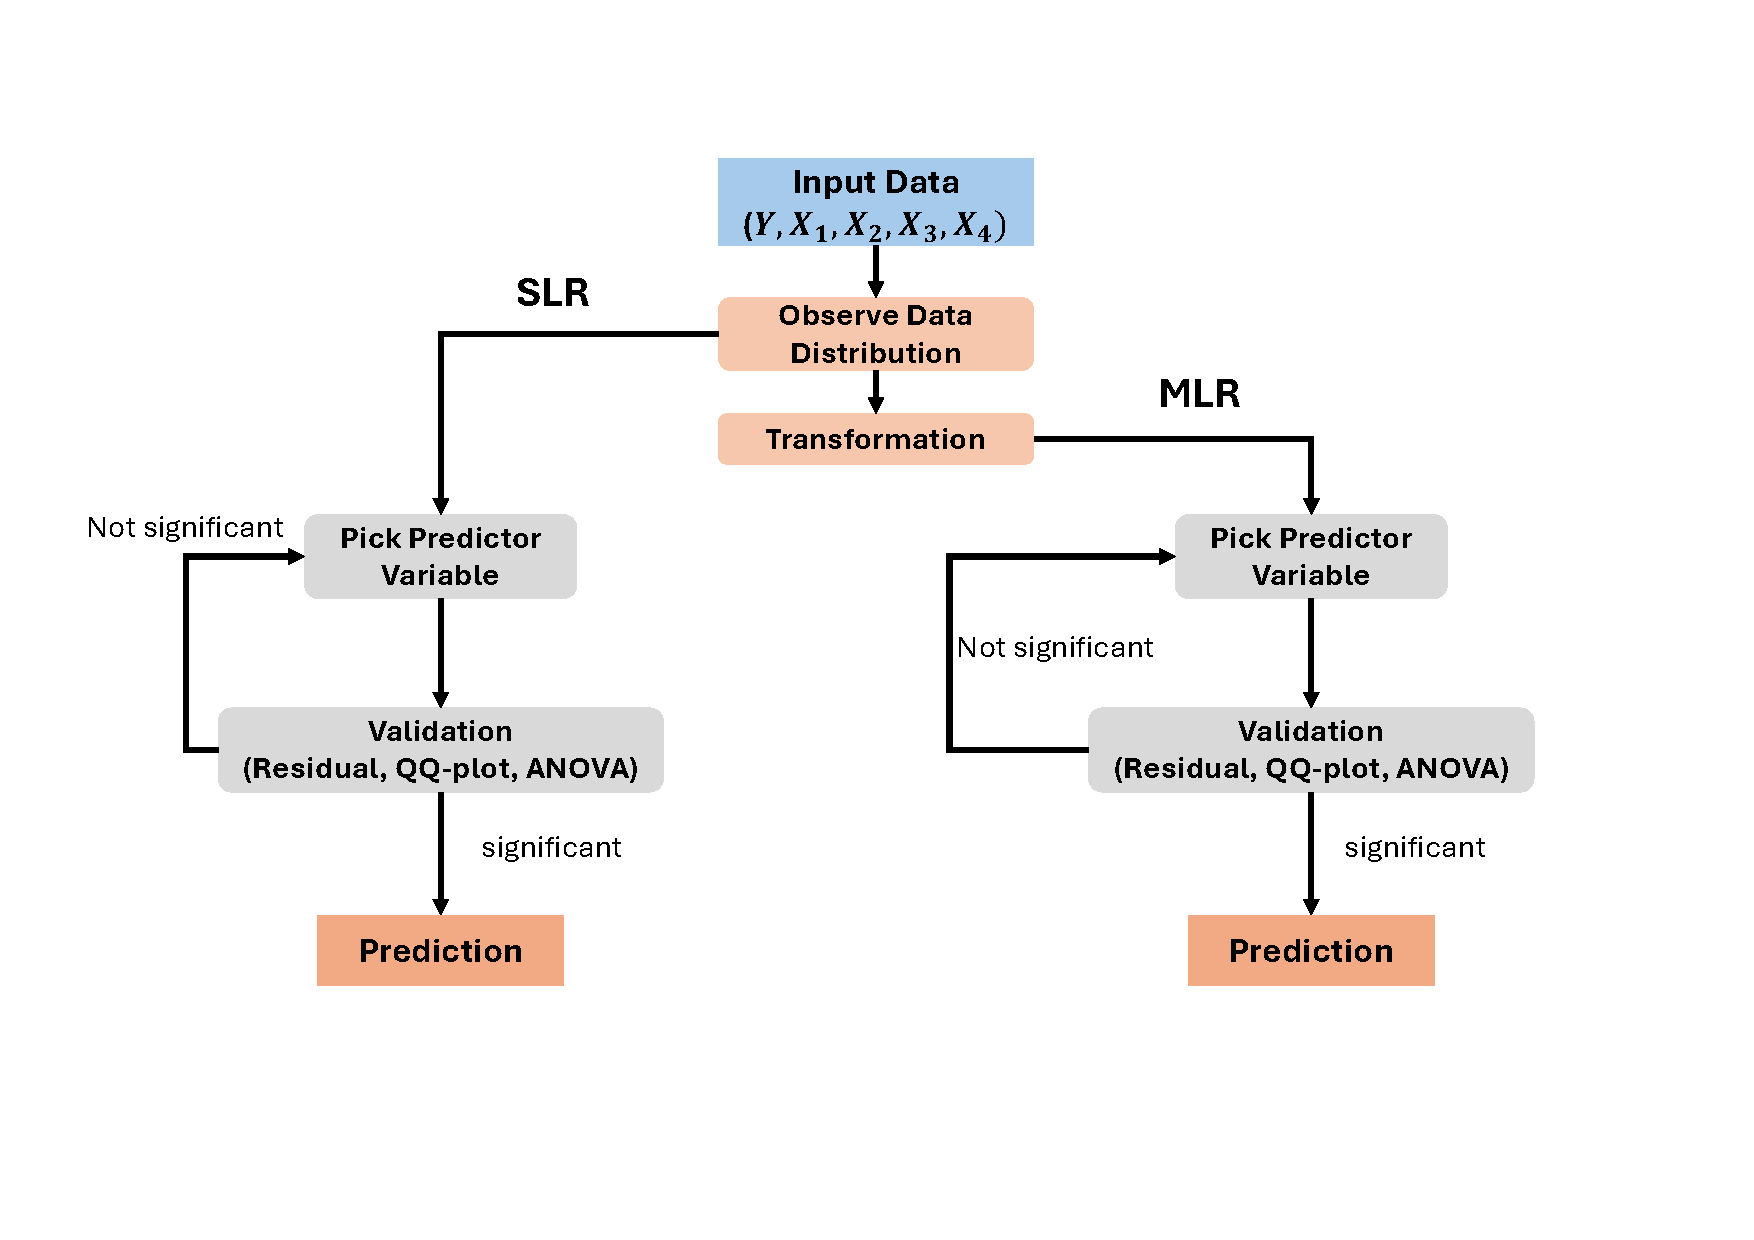
\includegraphics[width=1\linewidth]{figures/Intro.pdf}
    \caption{An overview of our pipeline.}
    \label{fig:intro}
\end{figure}

% 这部分就画画流程图,大概讲一下我们的流程
% 主要大概就是 overview -> slr -> mlr

\section{Dataset Overview and Representation}

The dataset is constituted of $5$ columns, with meaning shown in Table \ref{tab:variable_overview}. And Figure \ref{fig:single-data-analysis} illustrates the distributions of all variables.

In Figure \ref{fig:single-data-analysis}, it is clear that $y$ is left-skewed. We consider setting \begin{equation}
    y' = \log^2 y
\end{equation} to fix the skewness of the response variable. Equation 

\begin{figure}
    \centering
    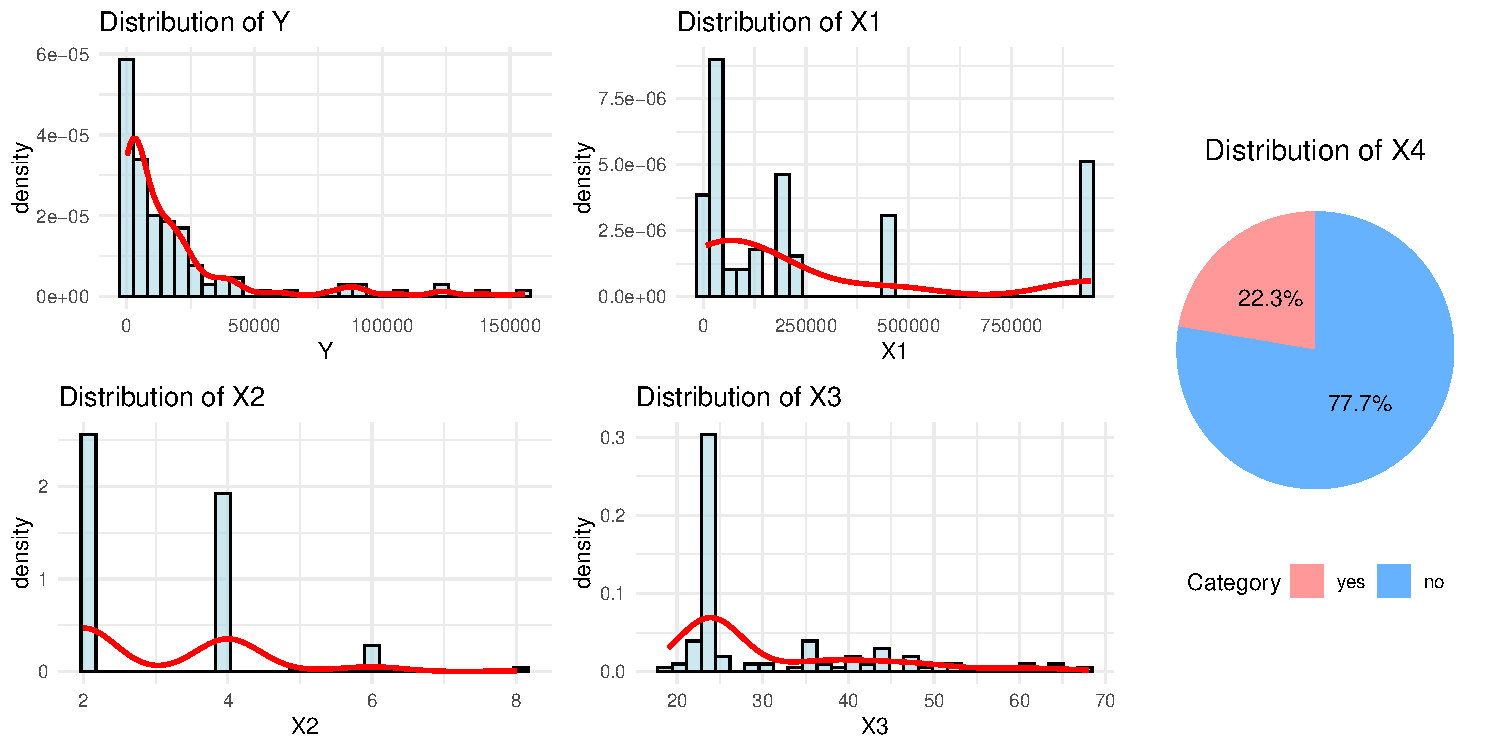
\includegraphics[width=1\linewidth]{figures/single_data_analysis}
    \caption{Distribution of the Variables}
    \label{fig:single-data-analysis}
\end{figure}

\begin{table}[t]
    \centering
    \begin{tabular}{c|l|l}
    \toprule
        \textbf{Columns} & \textbf{Meaning} & \textbf{Type}\\
        \midrule
        $y$ & Annual average daily traffic (AADT) & Continuous\\
        $x_1$ & Population of county in which road section in located & Discrete\\
        $x_2$ & Number of lanes in road section & Discrete\\
        $x_3$ & width of road section (in feet) & Continuous\\
        $x_4$ & Whether there is control of access to road section\tablefootnote{ $x_4 = 1$ means access control; $x_4 = 2$ means no access control} & Binary\\
    \bottomrule
    \end{tabular}
    \caption{Overview of the Variables}
    \label{tab:variable_overview}
\end{table}

In further analysis, we will use $y'$ as the response variable. To predict the value of $y$, we can easily do inverse transformation $y = \exp{\sqrt{y'}}$ to get the result.


Similarly, to fix the skewness of $x_1$, transformations are performed to $x_1$ with
\begin{equation}
x_1' = \sqrt{x_1}
\end{equation}

\begin{figure}
    \centering
    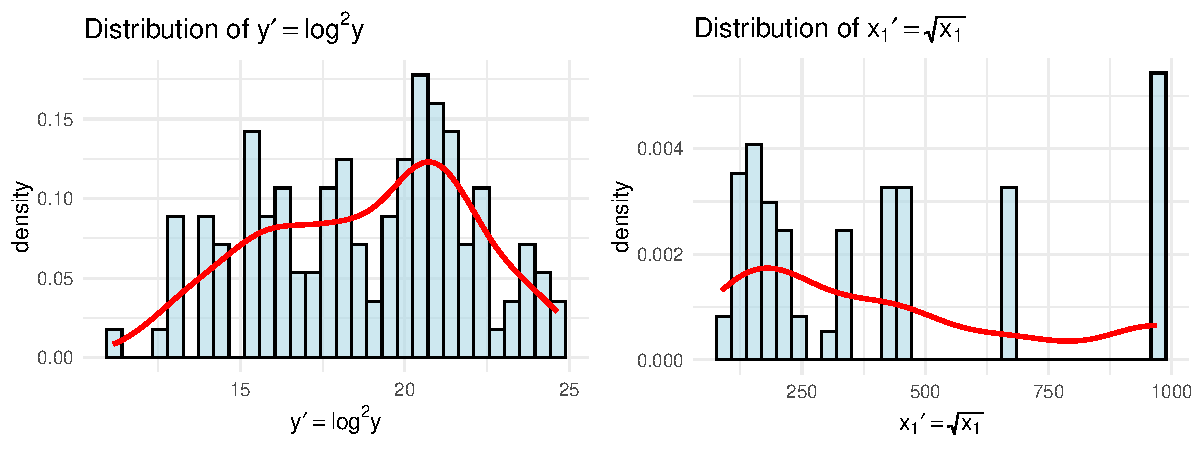
\includegraphics[width=1\linewidth]{figures/transformed_variables}
    \caption{Distribution of variables after transformation}
    \label{fig:transformed_variables}
\end{figure}

Figure \ref{fig:transformed_variables} shows the distribution of $y'$ and $x_1$, it can be seen that the distributions of $y'$ and $x_1'$ are relatively uniform compared with the original $y$ and $x_1$.

Although \( x_2 \) and \( x_3 \) also have some skewness, considering that they are integers\footnote{Although \( x_3 \) is defined as a continuous variable, it consists entirely of integers in the dataset.} with a small range in the dataset, applying a transformation may not be useful. We have decided not to transform them for now.

% For easier representation, we define the predictor as



\section{Single Variable Regression Analysis}

% 这个部分其实也不能叫 slr,所以我取了这样个名字。主要是第四个变量是二分类的。那就是前三个变量 slr 一下,然后最后一个就直接搞搞 anova 就行
% 可能每个都要配凑一下 transformation
% 图的话咱就这几个图:
% 对于不 transformation 和 trans 的应该都要画,一个是 scatter plot,一个大图就行。然后还有就是 fit 之后 res plot 那图,用灰色画一下那个 eps
% 然后每个可能都要做个 ANOVA

\subsection{Population v.s. AADT}

According to common sense, cities with larger populations should have more congested traffic. We attempt to use data to verify this hypothesis. 

\subsubsection{Model Overview}

By transforming \(x_1\) to \(\sqrt{x_1}\) and \(y\) to \(\log^2 y\), we ensured that potential non-linear relationships were better captured in the model.

\begin{figure}
    \centering
    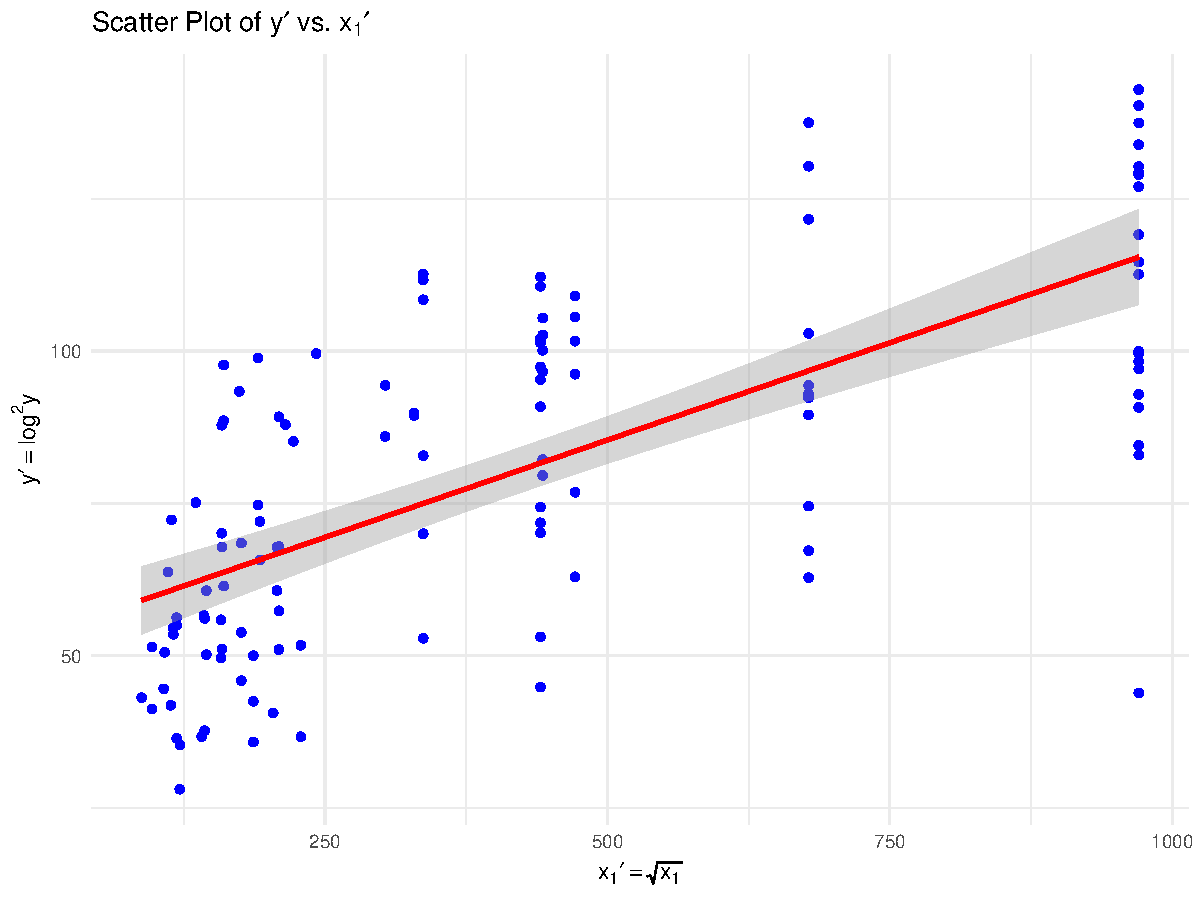
\includegraphics[width=0.5\linewidth]{figures/x1/scatter_plot}
    \caption{Scatter plot of the model $y' = \beta_0^{(1)} +\beta_1^{(1)} x_1' + \epsilon$}
    \label{fig:x1_scatter}
\end{figure}

\begin{figure}
    \centering
    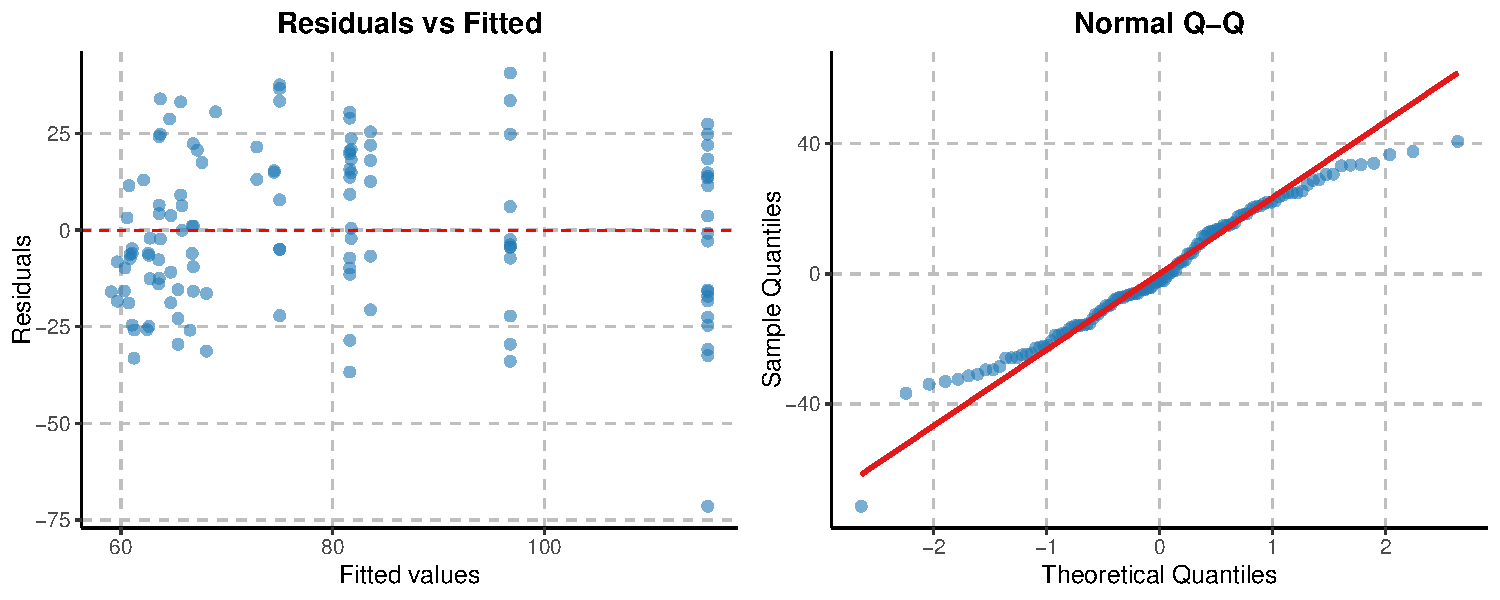
\includegraphics[width=1\linewidth]{figures/x1/residuals_vs_fitted_qqplot}
    \caption{Residuals of the model $\hat{y'} = \hat{\beta}_0^{(1)} +\hat{\beta}_1^{(1)} x_1'$}
    \label{fig:x1_res}
\end{figure}

We build a single linear regression model:
\begin{equation}
\begin{aligned}
y' = \beta_0^{(1)} + \beta_1^{(1)} x_1' + \epsilon, && \epsilon\sim\mathcal{N}(0, \sigma_1^2)
\end{aligned}
\end{equation}

%Figure \ref{fig:x1_res} % 写一下表示已经 insert 了,之后拿来直接用就行

The model is fitted with the data in figure , with 
\begin{equation}
    \begin{cases}
        \beta_0^{(1)}\approx 53.49\\
        \beta_1^{(1)}\approx 0.064
    \end{cases}
\end{equation}

This finding implies that larger county populations are associated with higher average annual daily traffic, which aligns with real-world expectations where more populated counties tend to have higher traffic volumes.

\subsubsection{Residuals Analysis}

We draw the residuals plot and QQ-plot in Figure \ref{fig:x1_res} to provide further insights into the model's adequacy.

\paragraph{Residuals Plot} The residual plot in Figure \ref{fig:x1_res} shows a generally even distribution of residuals around zero, though there are some signs of non-constant variance. This pattern might indicate that variability in traffic increases with larger predicted values, potentially due to factors such as urban infrastructure or public transport usage that could influence traffic in larger counties.

\paragraph{QQ-Plot} The QQ-plot of residuals shows that the residuals mostly follow a normal distribution, with minor deviations at the tails, suggesting that while the model performs well overall, there might be outliers or specific population segments where the prediction is less accurate.

\subsubsection{Residual Statistics}

\paragraph{ANOVA Table} We calculate the ANOVA table in Table \ref{tab:x1_anova}.

\begin{table}[ht]
    \centering
    \begin{tabular}{l|l|l|l|l}
    \toprule
        \textbf{Source} & \textbf{df} & \textbf{SS} & \textbf{MS} & $\mathcal{F}$ \\
        \midrule
        Regression & $1$ & $\mathrm{SSR} = 43471$ & $\mathrm{MS}_{\mathrm{Reg}} = \mathrm{SSR} = 43471$ & \multirow{2}{*}{$F = \frac{\mathrm{MS}_{\mathrm{Reg}}}{s^2} \approx 102.75$} \\
        Residual & $n - 2 = 119$ & $\mathrm{SSE} = 53916$ & $s^2 = \frac{\mathrm{SSE}}{n - 2} = 423$ & \\
        \midrule
        Total & $n - 1 = 120$ & $S_{yy} = 97387$ & & \\
    \bottomrule
    \end{tabular}
    \caption{ANOVA table for the population with AADT.}
    \label{tab:x1_anova}
\end{table}

Since $F$ value is in a $\mathcal{F}$ distribution:
\begin{equation}\label{eq:f_test}
    F = \frac{\mathrm{MS}_{\mathrm{Reg}}}{s^2}\sim \mathcal{F}_{1, n - 2}
\end{equation}

We can build $\mathcal{H}_0$: $\beta_1=0$ with $\mathcal{H}_1$: $\beta_1\neq 0$. And do $\mathcal{F}$-test by calculating the $p$ value:
\begin{equation}
    p = \mathbb{P}\left(\mathcal{F}_{1, 199} > F\right) < 2\times 10^{-16}
\end{equation}

The $p$ value is small enough for us to reject $\mathcal{H}_0$ and conclude that the population actually has a influence to AADT.

\paragraph{$\mathcal{R}^2$ Statistic} The $\mathcal{R}^2$ statistic is calculated as
\begin{equation}
    \mathcal{R}^2=\frac{\mathrm{SSR}}{S_{yy}}\approx 0.4634
\end{equation}

This means that while there is some relation between population and AADT, there are other effectors that determine the AADT.

\subsection{Number of Lanes v.s. AADT}

\begin{figure}
    \centering
    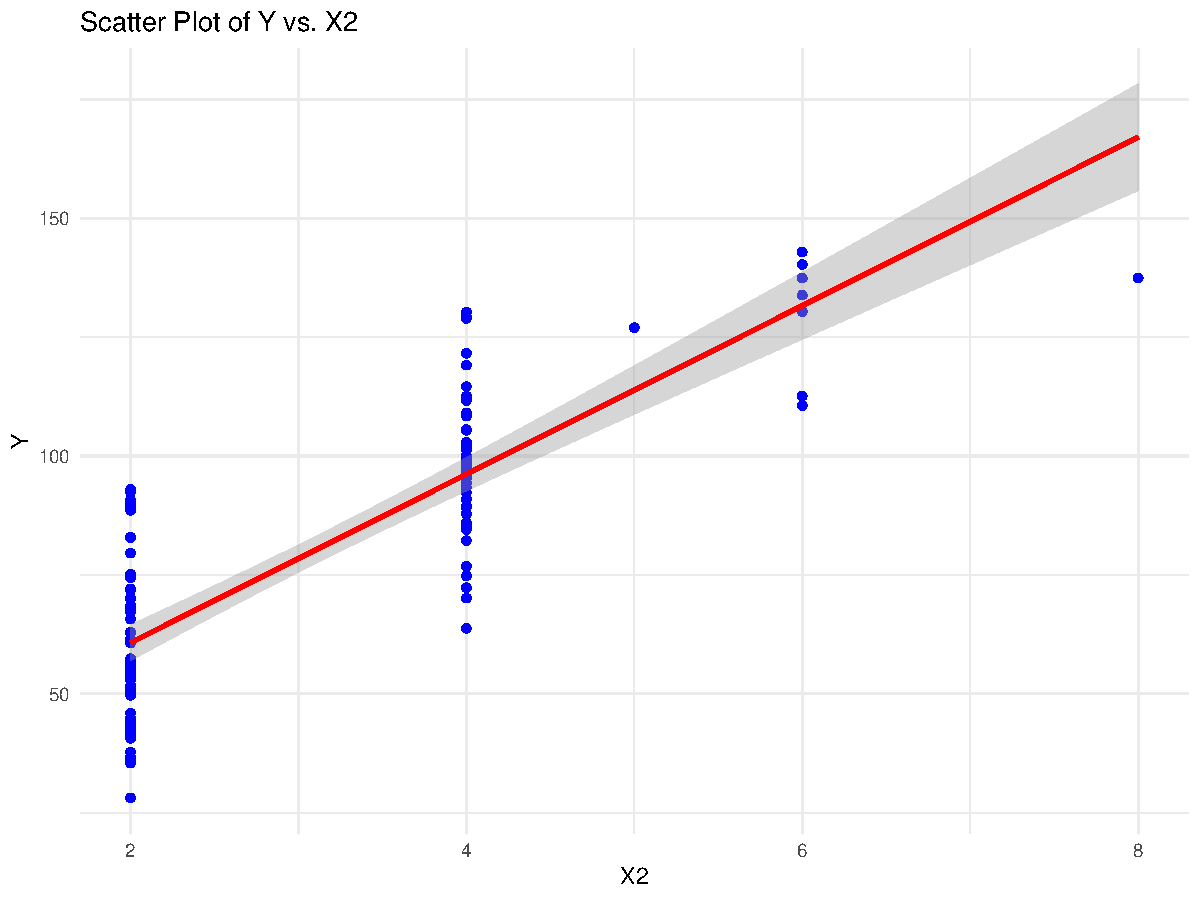
\includegraphics[width=0.5\linewidth]{figures/x2/scatter_plot}
    \caption{Scatter plot of the model $y' = \beta_0^{(2)} +\beta_1^{(2)} x_2' + \epsilon$}
    \label{fig:x2_scatter}
\end{figure}

\subsubsection{Model Overview}

The scatter plot Figure \ref{fig:x2_scatter} shows how AADT changes with the number of lanes. Each point represents a specific road section, with:
\begin{itemize}
    \item The $x$-axis representing the number of lanes.
    \item The $y$-axis representing the AADT data after transformation.
\end{itemize}

In this plot, we also include a trendline to indicate the general pattern in the data.

A positive slope in the trendline has been observed in the plot, which means that as the number of lanes increases, AADT tends to increase as well. This aligns with common sense: adding lanes generally allows a road to support more vehicles, which increases its traffic capacity.

We construct the linear model for the responsible variable $y'$ and predicted variable $x_2$:
\begin{equation}
\begin{aligned}
y' = \beta_0^{(2)} + \beta_1^{(2)} x_2 + \epsilon, && \epsilon\sim\mathcal{N}(0, \sigma_2^2)
\end{aligned}
\end{equation}

We fitted the model with the data, shown as the red line in Figure \ref{fig:x2_scatter}:
\begin{equation}
\begin{cases}
    \hat{\beta}_0^{(2)}\approx 25.304\\
    \hat{\beta}_1^{(2)}\approx 17.718
\end{cases}
\end{equation}

\paragraph{Intercept} When the number of lanes is zero, the model predicts $y'$ of approximately $25.3$. While this might not be meaningful practically (since we rarely see roads with zero lanes), it serves as a baseline.

\paragraph{Slope for \(x_2\)} For each additional lane, the model predicts an increase of about $17.7$ in $y'$. This means adding lanes has a significant positive effect on traffic capacity.

\paragraph{Significance} The very low $p$-value $\left(< 2\times 10^{-16}\right)$ for the number of lanes indicates that this relationship is statistically significant, implying that the number of lanes is an important factor in determining AADT.

\begin{figure}
    \centering
    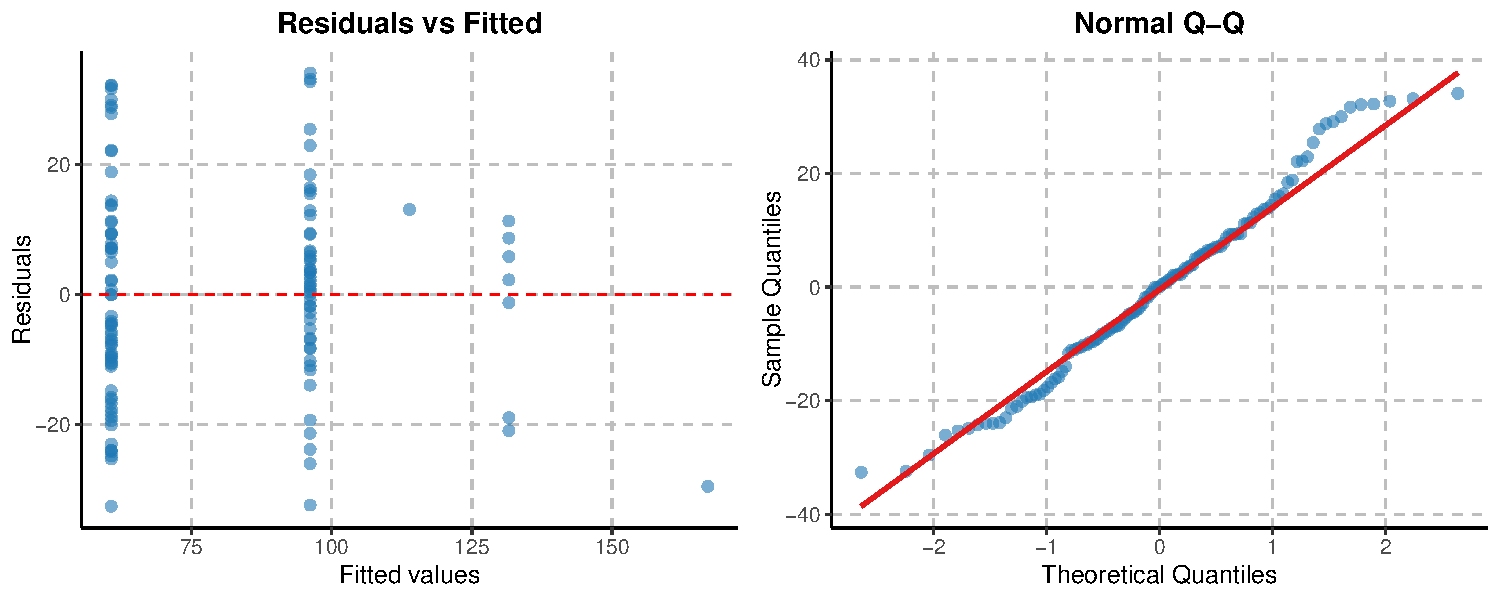
\includegraphics[width=1\linewidth]{figures/x2/residuals_vs_fitted_qqplot}
    \caption{Residuals of the model $\hat{y'} = \hat{\beta}_0^{(2)} +\hat{\beta}_1^{(2)} x_2$}
    \label{fig:x2_res}
\end{figure}

\subsubsection{Residual Analysis}

\paragraph{Residuals vs Fitted Plot} Figure \ref{fig:x2_res}  examines how well the linear model predicts AADT based on the number of lanes. If the residuals (the differences between actual and predicted AADT) are scattered randomly around the zero line, it indicates that the number of lanes effectively explains variations in AADT. In practical terms, this would mean that road sections with different lane counts generally show predictable changes in traffic volume, and our model captures this relationship well. However, if a pattern appears in the residuals, such as a consistent underestimation or overestimation of AADT for certain lane counts, it might suggest that factors beyond lane count (e.g., location, road type) are also influencing traffic volume, indicating that our model may need additional variables to improve accuracy.

\paragraph{Normal Q-Q Plot} Refer to  Figure \ref{fig:x2_res}  again, it assesses whether the residuals are normally distributed, which is an assumption for linear regression. A normal distribution of residuals suggests that the relationship between lane count and AADT is generally well-captured by the linear model. If the points fall along a straight line in the Q-Q plot, it indicates that the model’s errors are random and unbiased, meaning our predictions are reasonably reliable across different lane counts. However, significant deviations from this line might indicate that the relationship between lane count and AADT isn’t fully linear or that other factors are affecting traffic volume in ways the model doesn’t capture, possibly warranting a more complex or adjusted model.

\subsubsection{Residual Statistics}

\paragraph{ANOVA Table} We calculate the ANOVA table in Table \ref{tab:x2_anova}.

\begin{table}[ht]
    \centering
    \begin{tabular}{l|l|l|l|l}
    \toprule
        \textbf{Source} & \textbf{df} & \textbf{SS} & \textbf{MS} & $\mathcal{F}$ \\
        \midrule
        Regression & $1$ & $\mathrm{SSR} = 43471$ & $\mathrm{MS}_{\mathrm{Reg}} = \mathrm{SSR} = 43471$ & \multirow{2}{*}{$F = \frac{\mathrm{MS}_{\mathrm{Reg}}}{s^2} \approx 102.75$} \\
        Residual & $n - 2 = 119$ & $\mathrm{SSE} = 53916$ & $s^2 = \frac{\mathrm{SSE}}{n - 2} = 423$ & \\
        \midrule
        Total & $n - 1 = 120$ & $S_{yy} = 97387$ & & \\
    \bottomrule
    \end{tabular}
    \caption{ANOVA table for the population with AADT.}
    \label{tab:x2_anova}
\end{table}

According to Equation \ref{eq:f_test}, we can build $\mathcal{H}_0$: $\beta_1=0$ with $\mathcal{H}_1$: $\beta_1\neq 0$. And do $\mathcal{F}$-test by calculating the $p$ value:
\begin{equation}
    p = \mathbb{P}\left(\mathcal{F}_{1, 199} > F\right) < 2\times 10^{-16}
\end{equation}

The $p$ value is small enough for us to reject $\mathcal{H}_0$ and conclude that the population actually has a influence to AADT.

\paragraph{$\mathcal{R}^2$ Statistic} The $\mathcal{R}^2$ statistic is calculated as
\begin{equation}
    \mathcal{R}^2=\frac{\mathrm{SSR}}{S_{yy}}\approx 0.4634
\end{equation}

This means that while there is some relation between population and AADT, there are other effectors that determine the AADT.

\subsubsection{Summary}
This analysis shows that the number of lanes has a strong, positive effect on AADT. This makes intuitive sense, as wider roads with more lanes are better suited to handle larger volumes of traffic. The linear model and diagnostic plots suggest that the relationship is well captured by our model, with residuals generally behaving as expected.

In summary, as we add more lanes to a road, we can expect an increase in daily traffic capacity, which matches our common-sense understanding of road infrastructure and traffic flow.

\subsection{Road Width v.s. AADT}
\subsubsection{Model Overview}

We build the linear regression model
\begin{equation}
\begin{aligned}
y' = \beta_0^{(3)} + \beta_1^{(3)} x_3 + \epsilon, && \epsilon\sim\mathcal{N}(0, \sigma_3^2)
\end{aligned}
\end{equation}

The scatter plot in Figure \ref{fig:x3_scatter} shows the relationship between Annual Average Daily Traffic (AADT) and the width of road sections (in feet). Each point represents a specific road section, with:
The x-axis represents the width of the road section in feet \(x_3\).
The y-axis represents the AADT.

In this plot, a trendline has been added to indicate the general pattern in the data. Although the trendline suggests a positive slope, indicating that as the road width increases, AADT tends to increase, this relationship is not statistically significant, as shown by the linear model. 


\begin{itemize}

\item \textbf{Intercept}: 71.49, which suggests that at a hypothetical width of zero, the model would predict an AADT of approximately 71.5, though this does not have practical meaning.

\item \textbf{Slope for \(x_3\)}: 0.28, indicating a predicted increase in AADT of approximately 0.28 for each additional foot in road width. However, this effect is not statistically significant ($p$-value = 0.207), suggesting that road width does not significantly impact AADT in this model.
\end{itemize}

\begin{figure}
    \centering
    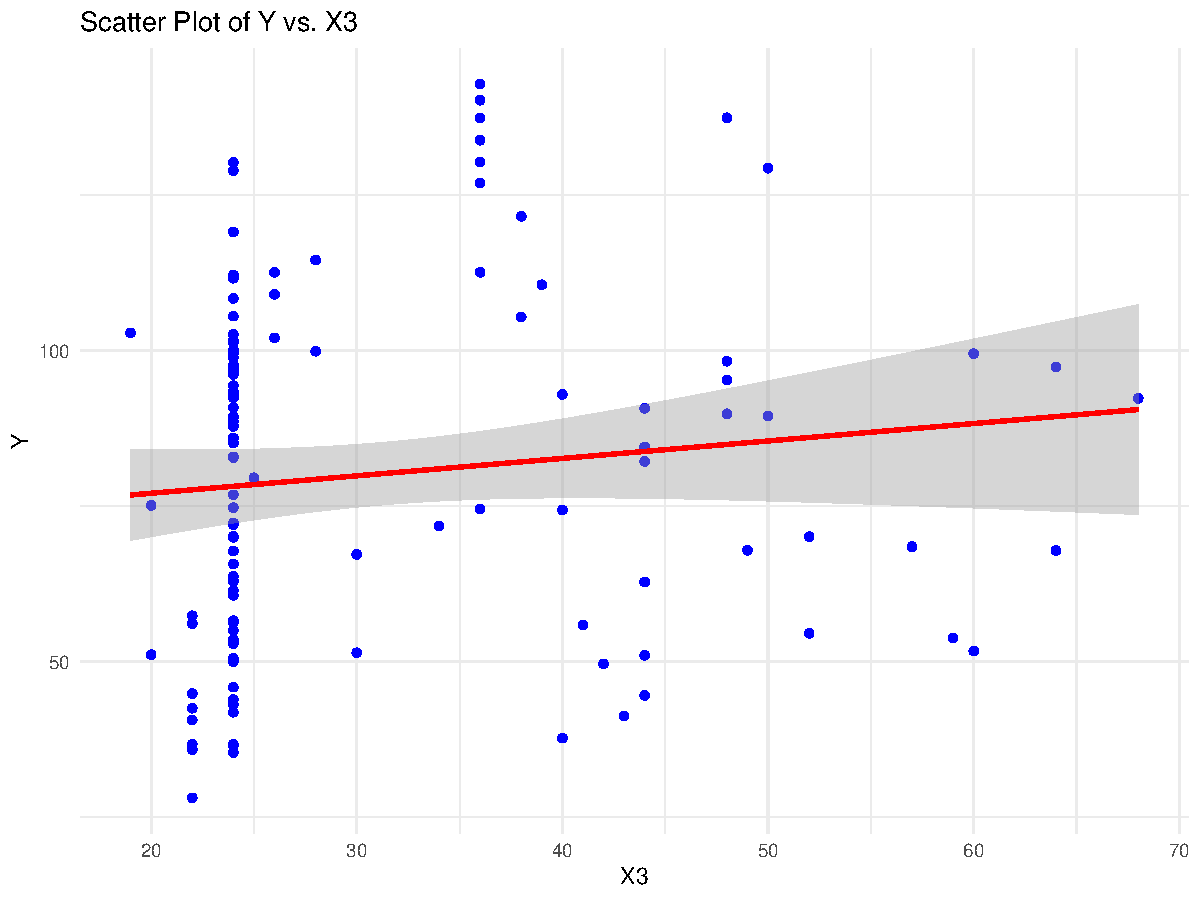
\includegraphics[width=0.5\linewidth]{figures/x3/scatter_plot}
    \caption{Residuals of the model $\hat{y'} = \hat{\beta}_0^{(3)} +\hat{\beta}_1^{(3)} x_3$}
    \label{fig:x3_scatter}
\end{figure}

\subsubsection{Residual Statistics}

\paragraph{ANOVA Table} We calculate the ANOVA table in Table \ref{tab:x3_anova}

\begin{table}[ht]
    \centering
    \begin{tabular}{l|l|l|l|l}
    \toprule
        \textbf{Source} & \textbf{df} & \textbf{SS} & \textbf{MS} & $\mathcal{F}$ \\
        \midrule
        Regression & $1$ & $\mathrm{SSR} =1254 $& $\mathrm{MS}_{\mathrm{Reg}} = \mathrm{SSR} = 1254.46$& \multirow{2}{*}{$F = \frac{\mathrm{MS}_{\mathrm{Reg}}}{s^2} \approx 1.6127$}\\
        Residual & $n - 2 = 119$ & $\mathrm{SSE} = 92564$& $s^2 = \frac{\mathrm{SSE}}{n - 2} = 777.85$& \\
        \midrule
        Total & $n - 1 = 120$ & $S_{yy} = 93818$& & \\
    \bottomrule
    \end{tabular}
    \caption{ANOVA table for the population with AADT.}
    \label{tab:x3_anova}
\end{table}

\paragraph{$\mathcal{R}^2$ Statistic} The $\mathcal{R}^2$ statistic is calculated as
\begin{equation}
    \mathcal{R}^2=\frac{\mathrm{SSR}}{S_{yy}}\approx 0.013
\end{equation}

implies that road width explains only about 1.3\% of the variation in AADT, suggesting that other factors are more influential.

\subsubsection{Summary}
This analysis suggests that the width of a road section has a weak and statistically insignificant relationship with AADT. While wider roads generally allow for higher traffic volumes, this model does not capture that effect effectively. 


\subsection{Whether to Control Access v.s. AADT}

Controlling access to the road section is one of the important methods for improving traffic flow. In this chapter, we explore whether this approach can effectively increase the annual average daily traffic.

We divide the data into two categories: the first category consists of data where control measures are implemented, and the second category consists of data without control measures. The distribution of these 2 categories is shown in Figure \ref{fig:x4_distribution}.

\begin{figure}
    \centering
    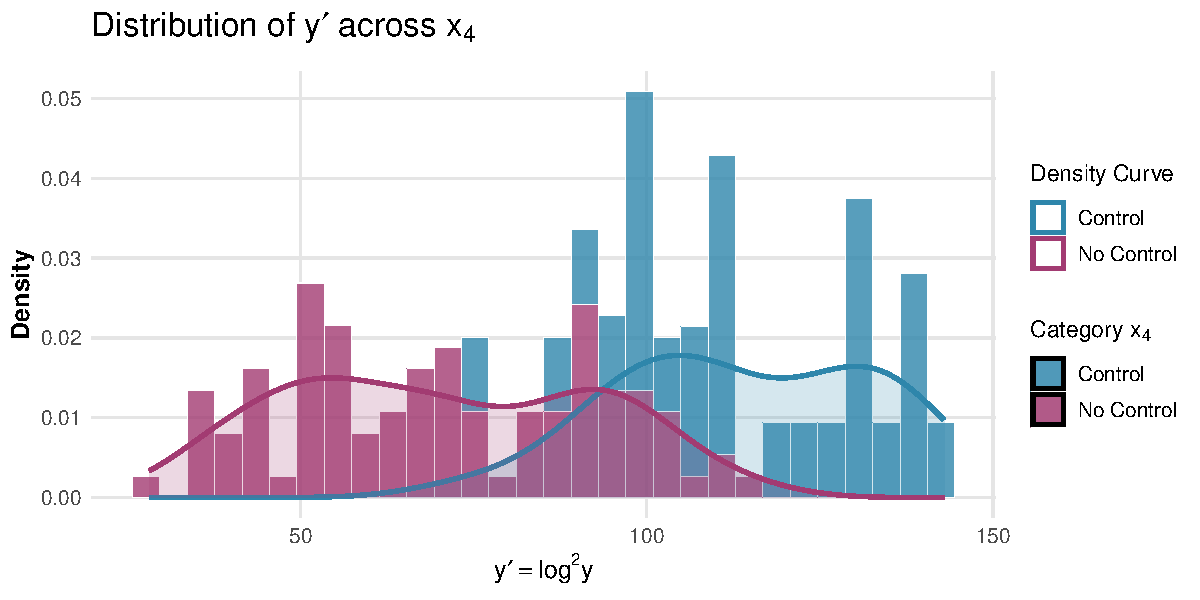
\includegraphics[width=1\linewidth]{figures/x4/histogram.pdf}
    \caption{Distribution of AADT over whether to control access.}
    \label{fig:x4_distribution}
\end{figure}

We then establish a linear model:
\begin{equation}
\begin{aligned}
y'_{ij} = \theta_i + \epsilon_{ij}, && i \in \{1, 2\}, j \in \left\{1, \cdots, n_i\right\}, && \epsilon_{ij}\sim \mathcal{N}\left(0, \sigma_4^2\right)
\end{aligned}
\end{equation}

We can fit the model by
\begin{equation}
    \begin{cases}
      \hat{\theta}_1 = \overline{y_{1\cdot}}\approx 114.10 \\
      \hat{\theta}_2 = \overline{y_{2\cdot}}\approx 70.48
    \end{cases}
\end{equation}

We are interested in whether these two categories have a significant difference. So we build $\mathcal{H}_0$: $\theta_1 = \theta_2$ versus $\mathcal{H}_1$: $\theta_1\neq\theta_2$, and we can build the ANOVA table, shown in Table \ref{tab:x4_anova}.

\begin{table}[ht]
    \centering
    \begin{tabular}{l|l|l|l|l}
    \toprule
        \textbf{Source} & \textbf{df} & \textbf{SS} & \textbf{MS} & $\mathcal{F}$ \\
        \midrule
        Between groups & $k - 1 = 1$ & $\mathrm{SST} = 39903$ & $\mathrm{MST} = \frac{\mathrm{SST}}{k - 1} = 39903$ & \multirow{2}{*}{$F = \frac{\mathrm{MST}}{\mathrm{MSE}} \approx 88.07$} \\
        Within groups & $n - k = 119$ & $\mathrm{SSE} = 53916$ & $\mathrm{MSE} = \frac{\mathrm{SSE}}{n - k} = 453$ & \\
        \midrule
        Total & $n - 1 = 120$ & $S_{yy} = 93819$ & & \\
    \bottomrule
    \end{tabular}
    \caption{ANOVA table for whether to control access.}
    \label{tab:x4_anova}
\end{table}

As
\begin{equation}
F = \frac{\mathrm{MST}}{\mathrm{MSE}} \sim \mathcal{F}_{1, 119}
\end{equation}

We can calculate $p$-value by:
\begin{equation}
p = \mathbb{P}\left(\mathcal{F}_{1, 199}>F\right)\approx 5.37\times 10^{-16}
\end{equation}

This is a quite small number, so we can conclude that there is a significant difference by controlling the access to the road section.

% 其实这里按道理应该做一个 non-parametric test,but i have no time...


\section{Multiple Linear Regression}

% 这段就搞个 ch7 的东西。然后可能要算算 SSE_omega - SSE_Omega 那种,对每个变量
% 最后也画画图,感觉可能有无 trans 都得整张
% 就是可能要解释一下那个第四个,用 t_4 = x_4 - 1 来代替(其实是一样的)

\subsection{Multiple Linear Regression with Full Dataset}

As $x_4$ is a classification variable, we create a \textit{dummy variable}
\begin{equation}
    x_4' = 2 - x_4
\end{equation}

So that $x_4 = 1$ means we select the first class (control) and $x_4 = 0$ means we select the second class.

So we can represent data by:
\begin{equation}
\begin{aligned}
\boldsymbol{x} = \begin{bmatrix}
    1\\x_1' \\ x_2 \\ x_3 \\ x_4'
\end{bmatrix}=\begin{bmatrix}
    1\\\sqrt{x_1} \\ x_2 \\ x_3 \\ 2 - x_4
\end{bmatrix}, && X = \begin{bmatrix}
    \boldsymbol{x_1}^\top \\ \boldsymbol{x_2}^\top \\ \vdots \\\boldsymbol{x_n}^\top
\end{bmatrix} = \begin{bmatrix}
    1 & x_{1,1}' & \ldots & x_{1,4}' \\ 1 & x_{2,1}' & \ldots & x_{2,4}' \\ \vdots & \vdots &\ddots &\vdots \\ 1 & x_{n,1}' & \ldots & x_{n,4}'
\end{bmatrix}
\end{aligned}
\end{equation}

And build the linear regression model for the full dataset:
\begin{equation} \label{eq:mlr}
    \log^2 y = \beta_0 +\beta_1 \sqrt{x_1} + \beta_2 x_2 +\beta_3 x_3 + \beta_4 (2 - x_4) + \epsilon = \boldsymbol{x}^\top\boldsymbol{\beta} + \epsilon
\end{equation}

We fit the model by
\begin{equation}
\hat{\beta} = (X^\top X)^{-1}Xy'\approx\begin{bmatrix}
    27.26 \\ 0.036 \\ 11.07 \\ 0.019 \\ -13.24
\end{bmatrix}
\end{equation}

\begin{figure}
    \centering
    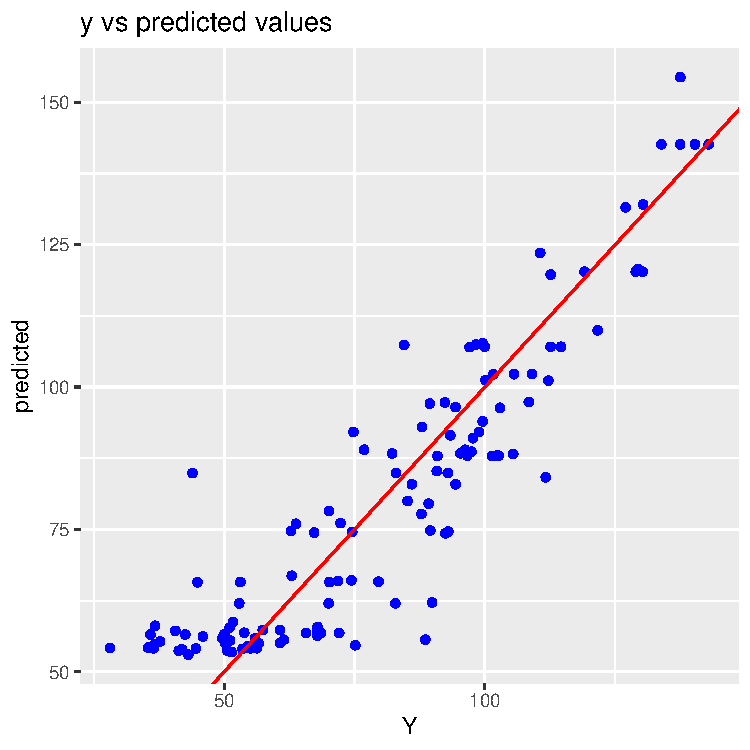
\includegraphics[width=0.5\linewidth]{figures/mlr/y_vs_predicted_values_full_model.pdf}
    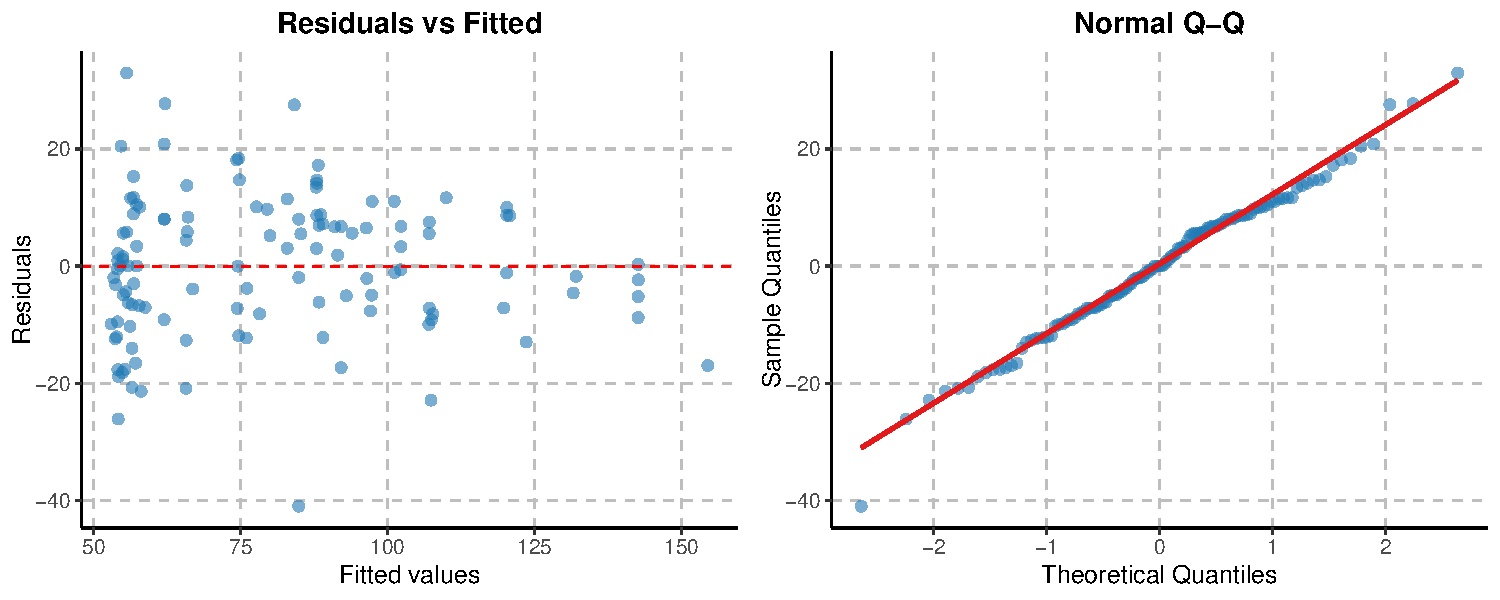
\includegraphics[width=1\linewidth]{figures/mlr/residuals_vs_fitted_qqplot.pdf}
    \caption{Regression model and residuals for the full model}
    \label{fig:full_mlr}
\end{figure}

\subsection{Adjusted Model}

Figure \ref{fig:full_mlr} shows the model prediction and residuals. We can find that the $\sigma$ of residuals are dependent with $y'$, so we need to adjust the transformation to make $\sigma$ a constant.

We succeed in the goal by doing the transformation
\begin{equation}\label{eq:trans_y_mlr}
y' = \log^4 y
\end{equation}

So the model becomes
\begin{equation}\label{eq:adjusted_model}
    \log^4 y = \beta_0 +\beta_1 \sqrt{x_1} + \beta_2 x_2 +\beta_3 x_3 + \beta_4 (2 - x_4) + \epsilon
\end{equation}

\begin{figure}
    \centering
    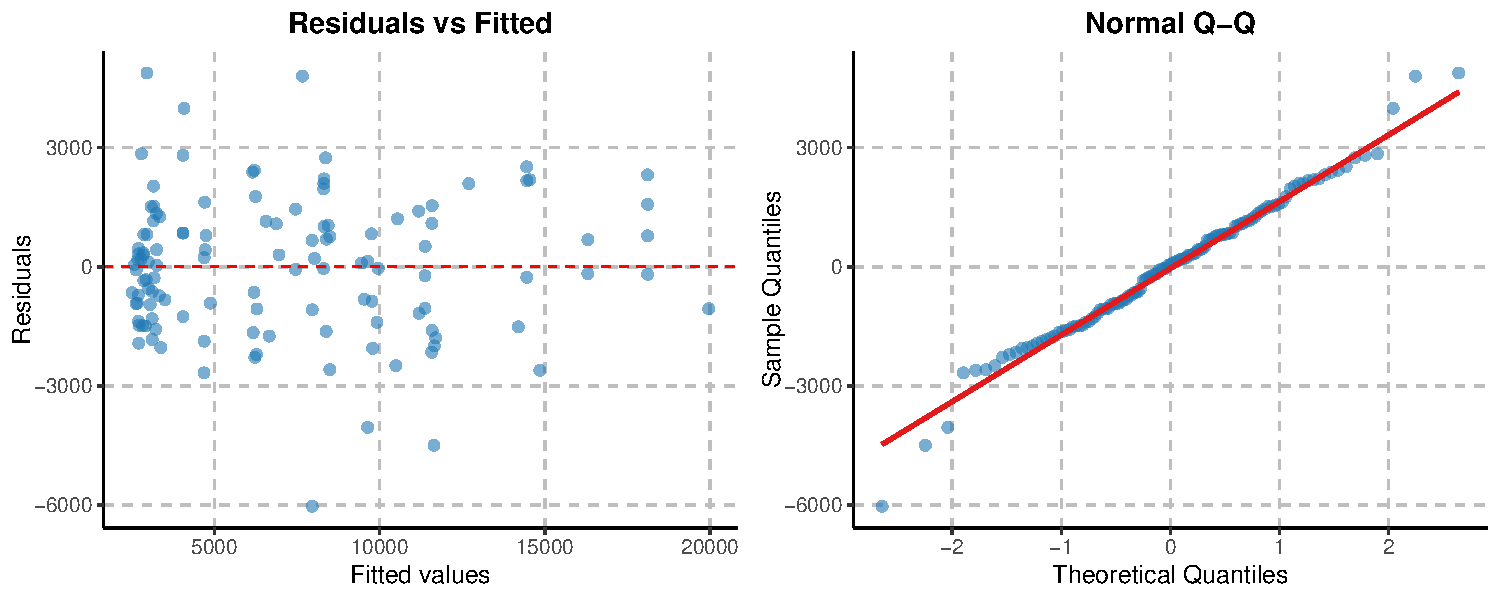
\includegraphics[width=1\linewidth]{figures/mlr/residuals_vs_fitted_qqplot_transformed.pdf}
    \caption{Regression model and residuals for the full model}
    \label{fig:adjust_mlr}
\end{figure}

Figure \ref{fig:adjust_mlr} shows residuals after adjustment. We can see that the $\sigma$ is mostly the same for each $y$.

\subsection{Adequacy Checking}

To check the adequacy of the model, we build an ANOVA / ANCOVA table for each variable. Shown in Table \ref{tab:mlr_anova}. We can find that $x_1', x_2, x_4'$ have information with $y$, while $x_3$ can be removed as it have a great $p$-value.

\begin{table}[ht]
    \centering
    \begin{tabular}{c|c|c|c|c}
    \toprule
        \textbf{Source} & \textbf{DF} & \textbf{RSS} & $\mathcal{F}$ & $p$-value \\
        \midrule
        Reduce $x_1$  & $117$ & $679542372$ & $99.815$ & $< 2.2\times 10^{-16}$\\
        Reduce $x_2$  & $117$ & $680342805$ & $100.07$ & $< 2.2\times 10^{-16}$\\
        Reduce $x_3$  & $117$ & $365429973$ & $0.0562$ & $0.8129$\\
        Reduce $x_4$  & $117$ & $459976649$ & $30.083$ & $2.457\times 10^{-7}$\\
        \midrule
        Full Model & $116$ & $365252858$ & & \\
    \bottomrule
    \end{tabular}
    \caption{ANOVA / ANCOVA table for adequacy checking.}
    \label{tab:mlr_anova}
\end{table}

So we decide to reduce $x_3$ from our model.

\subsection{Model Finalization}

So our final multiple linear regression model is 
\begin{equation}\label{eq:final_mlr}
    \log^4 y = \beta_0 +\beta_1 \sqrt{x_1} + \beta_2 x_2 +\beta_4 (2 - x_4) + \epsilon
\end{equation}

Figure \ref{fig:final_model} shows the predictions and residuals for the finalised model. We can observed that most of the residuals lie in the range $(-3000, 3000)$.

\begin{figure}
    \centering
    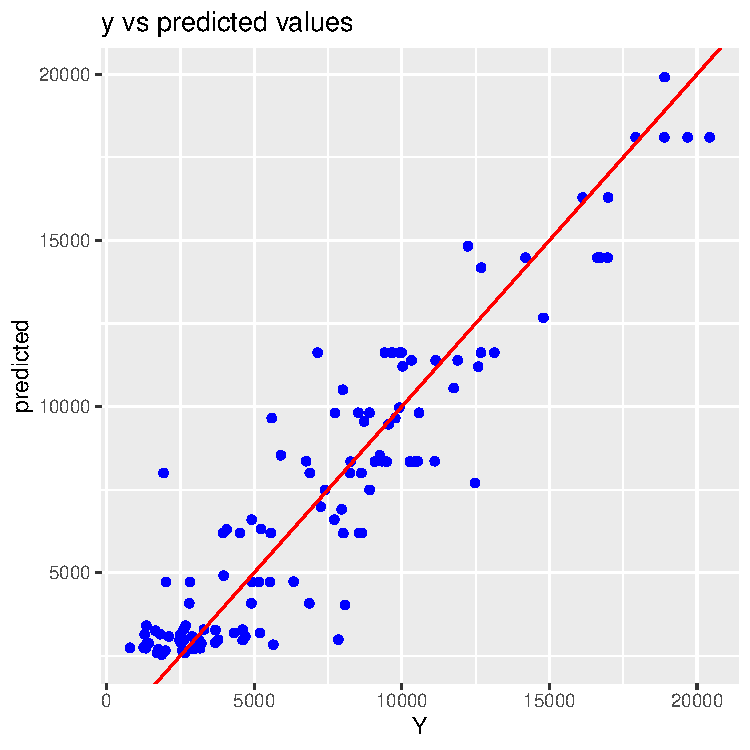
\includegraphics[width=0.5\linewidth]{figures/mlr/y_vs_predicted_values_reduced_model.pdf}
    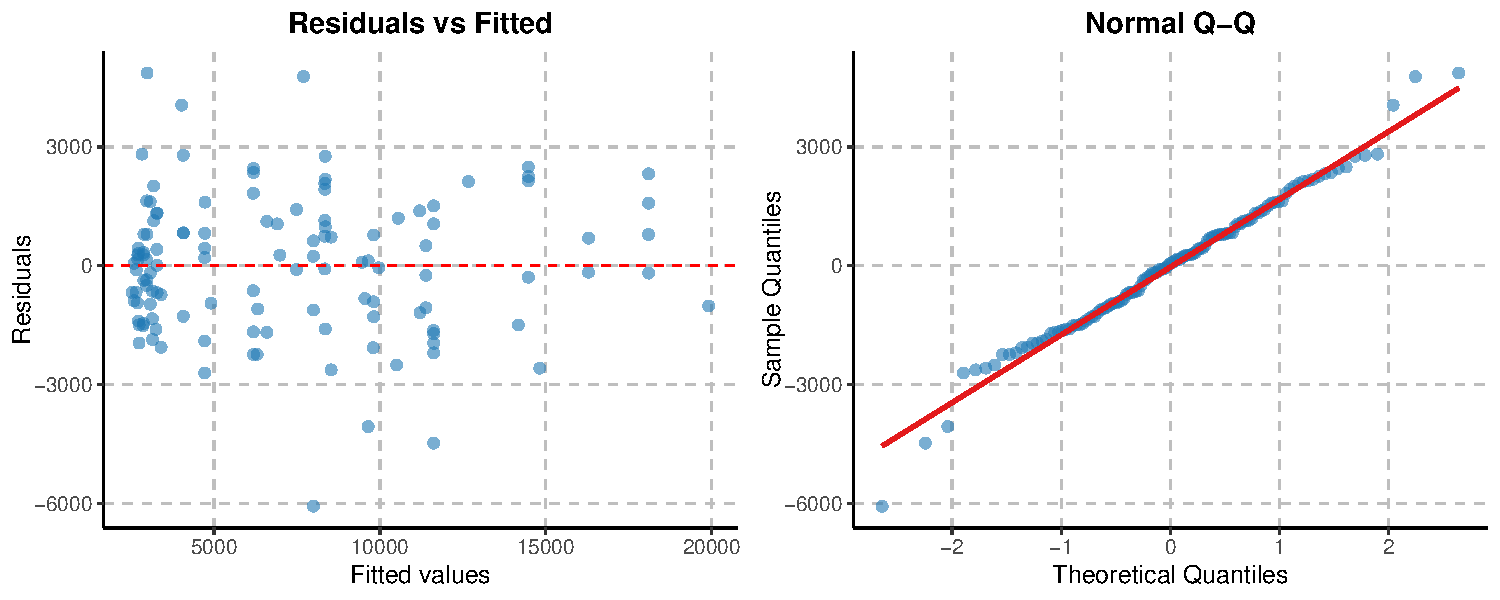
\includegraphics[width=1\linewidth]{figures/mlr/reduced_residuals_vs_fitted_qqplot.pdf}
    \caption{Predictions and residuals for the finalised model}
    \label{fig:final_model}
\end{figure}


\section{Prediction}

% 就把他最后一个 predict 一下,然后算算 conf interval 应该就问题不大了

\subsection{Point Estimation}

From Equation \ref{eq:final_mlr}, we can get:
\begin{equation}
    \hat{y} = \exp{\sqrt[4]{\hat{\beta}_0 +\hat{\beta}_1 \sqrt{x_1} + \hat{\beta}_2 x_2 + \hat{\beta}_4 (2 - x_4)}}
\end{equation}

Substituting by
\begin{equation}
\begin{cases}
x1 = 50000\\
x2 = 3\\
x3 = 60\\
x4 = 2\\
\end{cases}
\end{equation}

We can get
\begin{equation}\label{eq:prediction}
\hat{y}\approx 27379.73
\end{equation}

\subsection{Interval Estimation}

We can get the $90\%$ confidence interval of $\hat{y}'$:
\begin{equation}
    (l', r') = (9329.20, 12468.89)
\end{equation}

So after doing the inverse function of Equation \ref{eq:trans_y_mlr}:
\begin{equation}
y = \exp\sqrt[4]{y'}
\end{equation}

We can get the $90\%$ confidence interval:
\begin{equation}\label{eq:conf}
    (l, r) = (18544.14, 38836.96)
\end{equation}

\section{Conclusion}

Our single variable regression analysis showed that population size and the number of lanes significantly predict AADT, consistent with expectations that larger populations and additional lanes increase traffic capacity. However, road width was found to have a weak and statistically insignificant relationship with AADT. Access control demonstrated a substantial impact on traffic, as shown through a two-group comparison where controlled access increased AADT.

In the multiple linear regression model, we incorporated these significant factors, refining our understanding of how they collectively influence traffic patterns. This comprehensive approach provides a clearer picture of the primary determinants of traffic volume and informs infrastructure planning decisions. 

And finally, we provide our prediction in Equation \ref{eq:prediction} and \ref{eq:conf}.


% \bibliographystyle{plain} % or another style like apalike, abbrvnat, etc.
% \bibliography{references/ref} % assumes you have a references.bib file

\newpage
\appendix

\section{Code Snips}\label{appendix:key_code}

The full code can be accessed in \url{https://pufanyi.github.io/MH3510-Project/}, here we listed some of the code snips.

\subsection{Data Loading}

\begin{lstlisting}
file <- "../assets/aadt.txt"
data_raw <- read.table(file, col.names = columns)
data_ori <- data_raw[, c("Y", "X1", "X2", "X3", "X4")]
\end{lstlisting}

\subsection{Data Transformation}

\begin{lstlisting}
y_prime <- log(data$Y)^2
x1_prime <- sqrt(data$X1)
# ... Analysis code here
data$Y <- log(data$Y)^2
\end{lstlisting}

\subsection{Single Linear Regression and Analysis}

We take $x_1$ as an example

\begin{lstlisting}
slr_X1 <- lm(y_prime ~ x1_prime, data = data)
summary(slr_X1)
anova(slr_X1)
\end{lstlisting}

\subsection{Multiple Linear Regression}

\begin{lstlisting}
data$Y <- data$Y^2 # Further transformation
data$X4 <- 2 - data$X4 # Dummy variable

mlr <- lm(Y ~ X1 + X2 + X3 + X4, data = data)
summary(mlr)

# check adequecy
eliminate_x1_mlr <- lm(Y ~ X2 + X3 + X4, data = data)
anova(eliminate_x1_mlr, mlr)
# ... check other variables

# reduce model
mlr <- eliminate_x3_mlr
\end{lstlisting}

\subsection{Estimation}\label{appendix:prediction}

\begin{lstlisting}
x1 <- 50000
x2 <- 3
x3 <- 60
x4 <- 2

# transformation
x1 <- sqrt(x1)
x4 <- 2 - x4

# prediction
input <- data.frame(X1 = x1, X2 = x2, X3 = x3, X4 = x4)
y_hat <- predict(mlr, input)

# transform back
y_hat <- exp(y_hat^(1 / 4))

# interval estimation
alpha <- 0.1
interval <- predict(mlr, input, interval = "confidence", 
                    level = 1 - alpha)

# transform back
l <- exp(interval[2]^(1 / 4))
r <- exp(interval[3]^(1 / 4))
print(paste("(", l, ", ", r, ")"))
\end{lstlisting}



\end{document}